\chapter{Анализ секретности системы квантовой коммуникации с недоверенным приемным узлом} \label{ch:ch6}
\section{Исследование возможностей злоумышленника по получению информации о квантовом состоянии при разделении многофотонных состояний} \label{sec:ch6/sec1}

Пусть $|\alpha e^{i \varphi}\rangle$ - слабое когерентное состояниие, где $\alpha$ - это амплитуда состояния, а $\varphi$ - фаза, с помощью которой кодируется бит. Вероятность наблюдения ожидаемого результата измерения, говорящего о наличии $n$ фотонов в данном примере или импульсе, может быть получена с учетом следа продукта матрицы плотности когерентного состояния $\rho$ и проектора на Фоковский базис $|n\rangle\langle n|$: 
%
\begin{align}
    P_n&=\text{Tr}(\rho |n\rangle\langle n|) = \text{Tr}(|\alpha e^{i \varphi}\rangle \langle\alpha e^{i \varphi} |n\rangle\langle n|) \nonumber \\
    &= \text{Tr}(\sum_{k=0}^{\infty}\sum_{m=0}^{\infty} e^{-|\alpha|^2} \frac{(\alpha e^{i \varphi})^k(\alpha^{*} e^{-i \varphi})^m}{\sqrt{k!m!}} |k\rangle\langle m |n\rangle\langle n|) \nonumber  \\
    &=\sum_{j=0}^{\infty}\sum_{k=0}^{\infty}\sum_{m=0}^{\infty} e^{-|\alpha|^2} \frac{(\alpha e^{i \varphi})^k(\alpha^{*} e^{-i \varphi})^m}{\sqrt{k!m!}}\langle j |k\rangle\langle m |n\rangle\langle n|j\rangle \nonumber  \\
    &=e^{-|\alpha|^2} \frac{(|\alpha|^{2n})}{n!}, \label{pnver}
\end{align}
% 
где мы используем свойство ортогональности векторов Фоковского базиса $\langle k| n \rangle = \delta_{kn}$, где $\delta_{kn}$ - дельта-символ Кронекера. Таким образом, мы можем представить слабое когерентное состояние в Фоковском базисе, как:
%
\begin{equation}
    |\alpha e^{i \varphi}\rangle = e^{-\frac{|\alpha|^2}{2}}\sum_{n=0}^{\infty}  \frac{(\alpha e^{i \varphi})^n}{\sqrt{n!}} |n\rangle.
\end{equation}
%
Следовательно, состояние после измерения может быть сокращено следующим образом:
%
\begin{equation}
    \Tilde{\rho}=\frac{\sqrt{|n\rangle\langle n|} |\alpha e^{i \varphi}\rangle \langle\alpha e^{i \varphi} | \sqrt{|n\rangle\langle n|}}{P_n}.
\end{equation}
%
Исследуем, как оператор $\sqrt{|n\rangle\langle n|}$ воздействует на вектор в Фоковском базисе $|m\rangle$, представляя его в виде ряда Тейлора. Рассмотрим два различных случая:
%
\begin{enumerate}
    \item $m \neq n$
    \begin{align}
        \sqrt{|n\rangle\langle n|}|m\rangle = \sum_{k=0}^{\infty} \frac{(-1)^k(2k)!}{(1-2k)(k!)^2 4^k}(|n\rangle\langle n|-\hat{I})^k|m\rangle ,
    \end{align}
    где $\hat{I}$ оператор тождества. Используя следующие свойства
    \begin{gather}
        \hat{I}|m\rangle=|m\rangle, \\
        (|n\rangle\langle n|)^k |m\rangle = (|n\rangle\langle n|)^{k-1} |n\rangle\langle n|m\rangle = 0,
    \end{gather}
    получаем
    \begin{align}
       \sqrt{|n\rangle\langle n|}|m\rangle = \sum_{k=0}^{\infty} \frac{(-1)^k(2k)!}{(1-2k)(k!)^2 4^k}(-1)^k|m\rangle = 0 |m\rangle.
    \end{align}
    \item $m=n$
    
   Затем, используя следующие свойства
    \begin{align}
        (|n\rangle\langle n|)^k |n\rangle = (|n\rangle\langle n|)^{k-1}=\nonumber\\ =|n\rangle\langle n|n\rangle = (|n\rangle\langle n|)^{k-1} |n\rangle = ... = |n\rangle,
    \end{align}
    тогда
    \begin{align}
        \sqrt{|n\rangle\langle n|}|n\rangle &= \sum_{k=0}^{\infty} \frac{(-1)^k(2k)!}{(1-2k)(k!)^2 4^k}(|n\rangle\langle n|-\hat{I})^k|n\rangle \nonumber\\
        &=|n\rangle + \sum_{k=1}^{\infty} \frac{(-1)^k(2k)!}{(1-2k)(k!)^2 4^k}(|n\rangle\langle n|-\hat{I})^k|n\rangle \nonumber\\
        &=|n\rangle + 0 = |n\rangle
    \end{align}
\end{enumerate}

Таким образом, в сокращенном виде:

\begin{equation}
	\begin{aligned}
   		\Tilde{\rho}&=\frac{1}{P_n}\sum_{k=0}^{\infty}\sum_{m=0}^{\infty} e^{-|\alpha|^2} \frac{(\alpha e^{i \varphi})^k(\alpha^{*} e^{-i \varphi})^m}{\sqrt{k!m!}} \sqrt{|n\rangle\langle n|}|k\rangle\langle m |\sqrt{|n\rangle\langle n|} \nonumber \\
  			 &= \frac{1}{P_n} P_n |n\rangle\langle n| = |n\rangle\langle n|	
  	 \label{rhored}
	\end{aligned}
\end{equation}

Тем самым, в соответствии с выражениями, полученными в \ref{pnver} и \ref{rhored} результат измерения числа фотонов в импульсе (проекция на Фоковский базис) в слабом когерентном импульсе и сокращенное состояние после измерения не содержат информации о фазе когерентного состояния $\varphi$. В случае с множеством мод, проблема сводится к случаю с одной модой, описанному выше.
\pagebreak

%%%%%%%%%%%%%%%%%%%%%%%%%%%%%%%%%%%%%%%%%%%%%%%%%%%%%%%%%%%%%%%%%%%%%%%%%%%%%%%%%
\section{Оценка скорости формирования секретного ключа в асимптотическом приближении} \label{ch:ch6/sec2}

Определим выражение для оценки средней скорости формирования просеянных ключей $C$ (идентичных битов у отправителя и получателя, но скоррелированных со злоумышленником, в связи с чем, требуется процедура усиления секретности) 
\begin{equation}
    C=FR(1-h(Q)),
\end{equation}
где $h(Q)$ - функция двоичной энтропии.

Чтобы оценить скорость формирования ключа мы используем общеизвестный метод, предложенный в \cite{devetak2005distillation}.

Оценка границы Холево для многомодовых когерентных состояний дана в \ref{phi} в соответствии с \cite{kozubov2019finite}:
\begin{equation}
    \chi=h\left(\frac{1-e^{-\mu_0(1-d^S_{00}(2\beta))}}{2}\right)\approx h\left(\frac{1-e^{-2\mu}}{2}\right).
\end{equation}

Она показывает максимальное количество информации, которую Ева может получить из состояний в одном канале. Однако, в схеме с недоверенным узлом используются два независимых канала. Следовательно, злоумышленник может осуществлять независимые измерения в двух квантовых каналах и получать следующее количество информации:
\begin{equation}
    \tilde{\chi}=2(1-\chi)\chi+\chi^2.
\end{equation}

Таким образом, асимптотическая скорость генерации кодирующей битовой последовательности $K$ будет следующим:
\begin{equation}
     K=FR(1-\xi h(Q)-\tilde{\chi}),
\end{equation}
где $\xi$ - эффективность процедуры исправления ошибок. 

Для расчетов возьмем экспериментальные параметры одного из режимов, использованных в \cite{Gleim16,Miroshnichenko18}, которые близки к экспериментальной реализации нашей модели: $F=100$ МГц, $\mu=0.1$, $\mu_0=4$, $\Delta\varphi=5^{\circ}$, $\vartheta=10^{-3}$, $\xi=1.15$, $\varphi_0=5^{\circ}$ $\eta_D=0.25$, $\gamma_{dark}= 10$ Гц. Расчетные результаты показаны на рисунке \ref{fig:fig2}.

\begin{figure}
	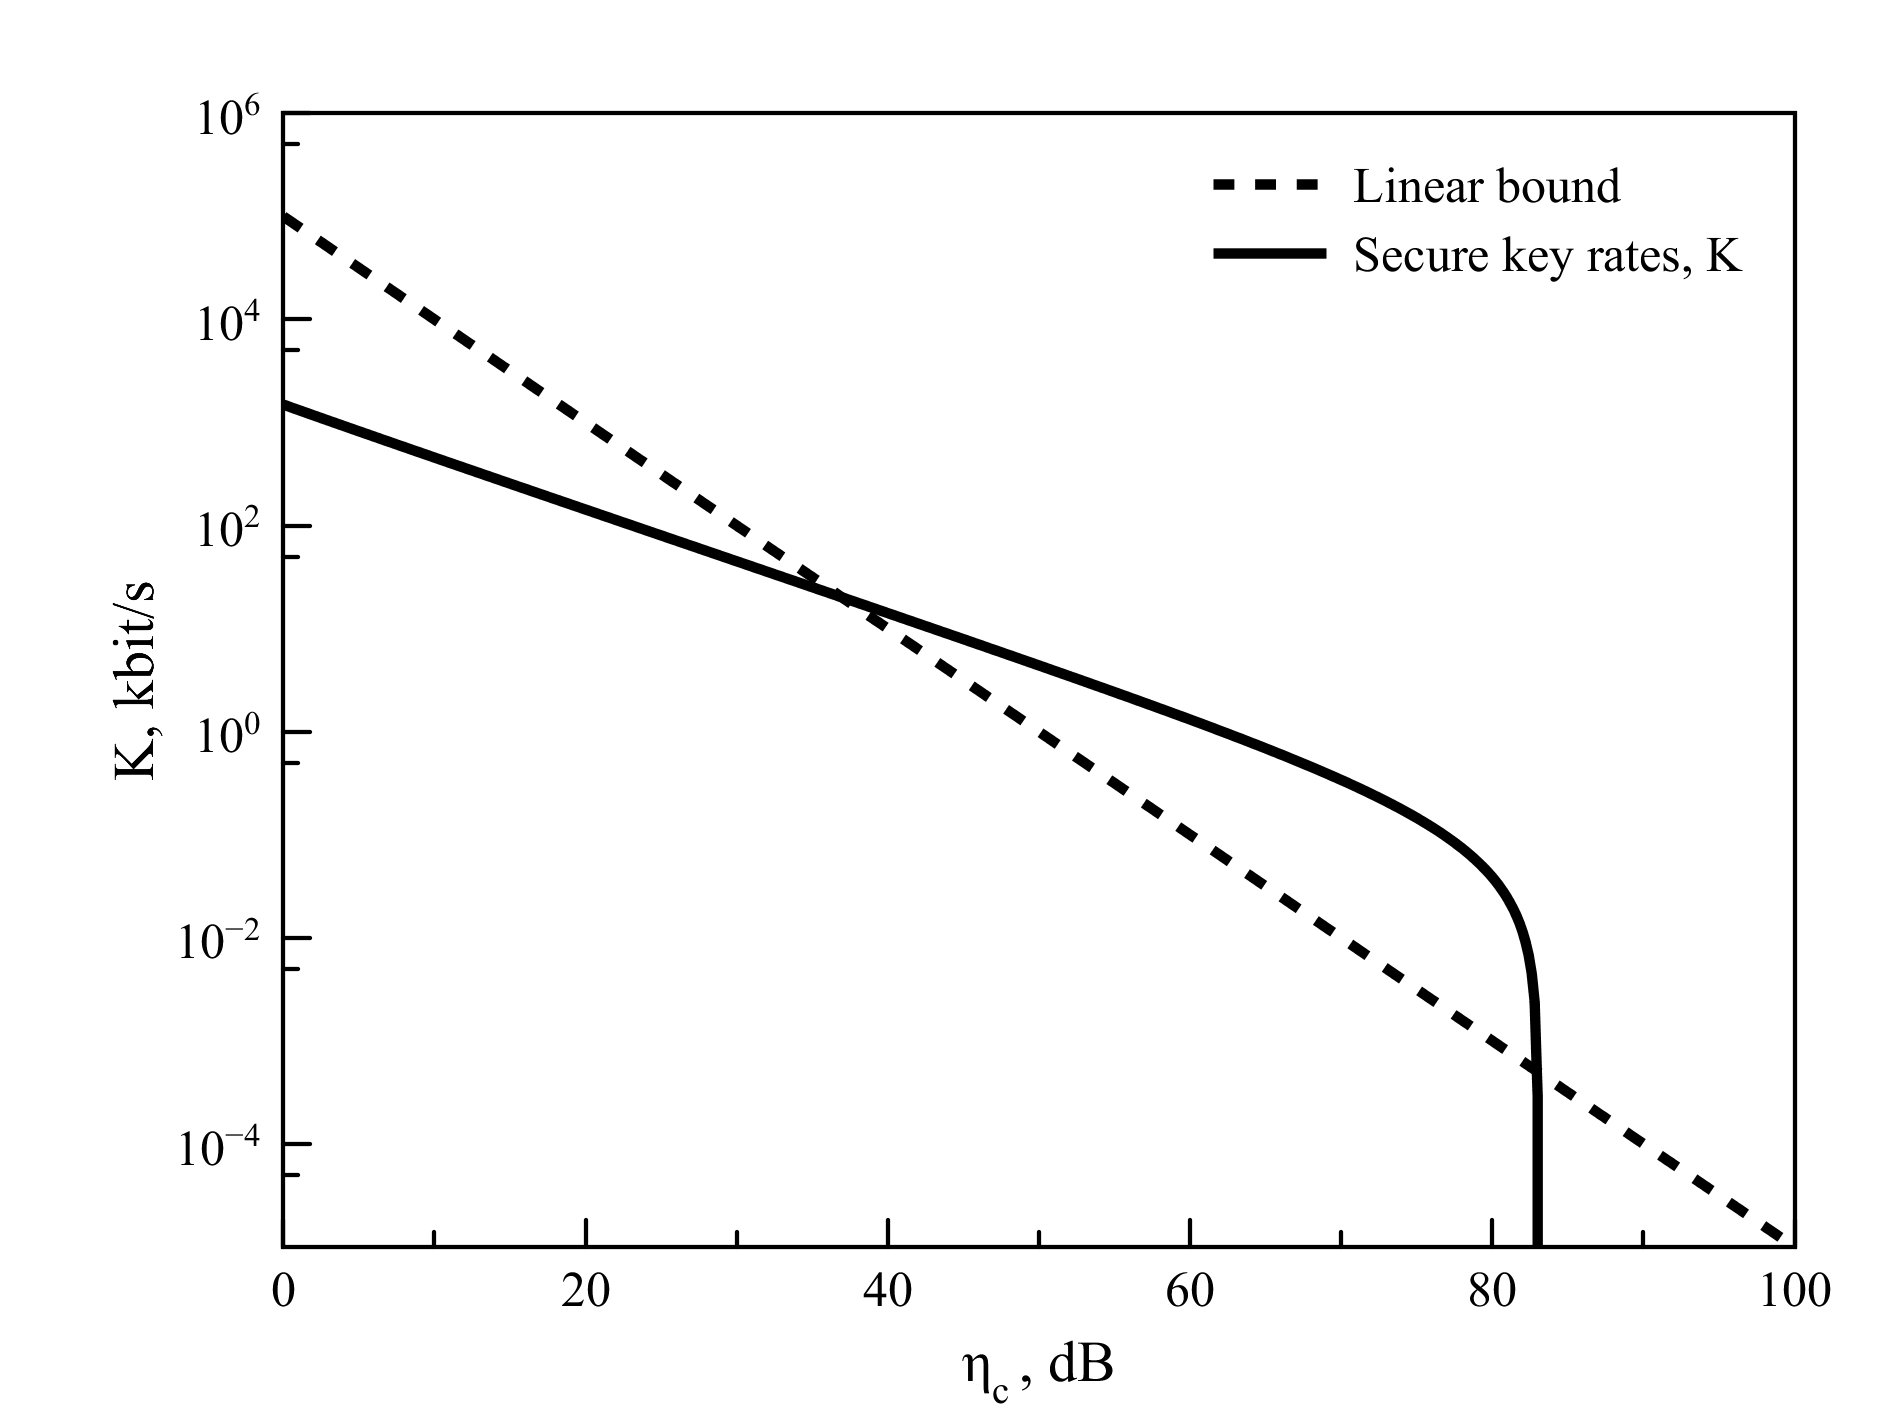
\includegraphics[width=1\linewidth]{TFQKD.png}
	\caption{Расчет параметров системы квантовой коммуникации на боковых частотах модулированного излучения с недоверенным узлом.}
	\label{fig:fig2}
\end{figure}

Для предполагаемых значений скорость формирования ключа превышает линейный предел скорости \cite{pirandola2017fundamental} где $\eta_c \gtrsim$ 40 дБ (200 км). Вдобавок, предлагаемый в работе протокол также способен достичь длины линии передачи $\eta_c\approx$ 83 дБ (460 км).

%Наконец, можно определить выражение для оценки среднего значения скорости формирования просеянного ключа $K$ (одинаковые биты между легитимными пользователями, но коррелирующие с возможным результатом у злоумышленника, что требует проведения процедуры усиления секретности)

%\begin{equation}
%   K=FR(1-h(Q)),
%\end{equation}
%где $h(Q)$ это функция двоичной энтропии. 

\pagebreak

%%%%%%%%%%%%%%%%%%%%%%%%%%%%%%%%%%%%%%%%%%%%%%%%%%%%%%%%%%%%%%%%%%%%%%%%%%%%%%%%%%
\section{Выводы по главе} \label{ch:ch6/sec3}
В главе показано, что для когерентных многомодовых квантовых состояний атака злоумышленника с разделением многофотонных состояний не приводит к раскрытию ключевой информации, так как при измерении числа фотонов в импульсе (проекции на Фоковский базис), сокращенное состояние не содержит информацию о фазе когерентного состояния. В главе приведена оценка скорости формирования просеянных ключей для системы с недоверенным узлом, в которой не учитывается доля информации, получаемая злоумышленником из квантового канала и после исправления ошибок. Также приведена оценка асимптотической скорости формирования ключа с учетом возможности получения ключевой информации из двух независимых каналов в системе с недоверенным приёмным узлом. Проведен расчет параметров системы с характеристиками из публикаций о системе квантовой коммуникации. В соотвествии с расчетом показано, что одним из преимуществ протокола с недоверенным узлом является превышение величины скорости формирования ключа над линейной границей в определенном диапазоне дистанций.



